%% ============================================================
%%  CHAPTER 1 — Introduction
%% ============================================================
\chapter{Introduction}
\label{ch:introduction}

\nomenclature{COMPAS}{Correctional Offender Management Profiling for Alternative Sanctions}
\nomenclature{KL}{Kullback--Leibler Divergence}
\nomenclature{CVaR}{Conditional Value-at-Risk}
\nomenclature{ELBO}{Evidence Lower Bound}
\nomenclature{AE}{Autoencoder}
\nomenclature{VAE}{Variational Autoencoder}
\nomenclature{TC}{Total Correlation}
\nomenclature{GAN}{Generative Adversarial Network}
\nomenclature{GRL}{Gradient Reversal Layer}
\nomenclature{FrFT}{Fractional Fourier Transform}
\nomenclature{FPR}{False Positive Rate}
\nomenclature{TPR}{True Positive Rate}
\nomenclature{EO}{Equal Opportunity}
\nomenclature{EOdd}{Equalized Odds}
\nomenclature{FD-VAE}{Fairness-aware Disentangling Variational Autoencoder}
\nomenclature{TAL}{Target Attribute Latent}
\nomenclature{PAL}{Protected Attribute Latent}
\nomenclature{MAL}{Mutual Attribute Latent}
\nomenclature{DAG}{Demographic-Agnostic}
\nomenclature{DAW}{Demographic-Aware}
\nomenclature{FDD}{Fair Deepfake Detection}
\nomenclature{DAG-FDD}{Demographic-Agnostic Fair Deepfake Detection}
\nomenclature{DAW-FDD}{Demographic-Aware Fair Deepfake Detection}
\nomenclature{FF++}{FaceForensics++}
\nomenclature{DFD}{DeepFakeDetection Dataset}
\nomenclature{DFDC}{DeepFake Detection Challenge Dataset}
\nomenclature{Celeb-DF}{Celeb DeepFake Dataset}
\nomenclature{DRO}{Distributionally Robust Optimization}
\nomenclature{GFPR}{Group False Positive Rate}
\nomenclature{FFPR}{False Positive Rate Disparity (Fairness FPR)}
\nomenclature{FEO}{Equalized Odds-based Fairness Metric}
\nomenclature{AUC}{Area Under the Curve}
\nomenclature{ACC}{Accuracy}
\nomenclature{FFVAE}{Fairness-aware Disentangling Variational Autoencoder (prior method)}
\nomenclature{DRL}{Disentangled Representation Learning}

Artificial intelligence has moved, in a remarkably short span of time, from
the edges of academic research into the operational core of institutions
that shape daily life.  Decisions about who receives a loan, who advances
past an automated resume screen, how a medical scan is flagged for review,
and whether a defendant is assessed as a recidivism risk are increasingly
mediated by learned models.  This transition has delivered genuine
efficiency gains, but it has also surfaced a set of ethical challenges
that the field was, for much of its early history, poorly equipped to
address.  Foremost among these is the question of fairness: whether the
errors that AI systems make are distributed uniformly across the population,
or concentrated disproportionately among groups that are already
disadvantaged.

This report examines the theoretical and algorithmic foundations of
fairness-aware machine learning, surveys the architectural approaches that
have emerged in response to demographic bias, and presents a pipeline that
combines several of these approaches for fair deepfake detection.  The
chapter proceeds from context and motivation through real-world case studies
to a discussion of methodological limitations and an overview of the report
structure.

% ,,,,,,,,,,,,,,,,--
\section{AI in Society: Scale and Stakes}
\label{sec:ai_growth}
% ,,,,,,,,,,,,,,,,--

The contemporary wave of AI is distinguished from earlier periods principally
by scale, of data, compute, and deployment.  Deep learning models that once
struggled to classify handwritten digits can now generate realistic images,
translate across dozens of languages, and diagnose pathologies from medical
images with accuracy comparable to specialist physicians.  These capabilities
have diffused rapidly into industry and government.  Recent surveys suggest
that over three-quarters of organisations worldwide have incorporated AI into
at least some operational processes~\cite{mckinsey2024}.

The domains of deployment are increasingly consequential.  Algorithmic credit
scoring evaluates loan applications at a scale and speed that human review
cannot match.  Hiring platforms use natural language processing to filter
thousands of resumes before a recruiter sees any candidate.  Law enforcement
agencies in several jurisdictions have deployed facial recognition and
recidivism prediction tools with direct implications for individual liberty.
Healthcare systems use predictive models to triage patients and flag
diagnostic anomalies.

What distinguishes these applications from earlier automation is a shift from
\emph{explicit rule specification} to \emph{implicit statistical learning}.
A rule-based system encodes its logic transparently and can be inspected
and revised.  A deep neural network trained on historical data encodes its
decision logic in millions of numerical parameters, learning from data that
may carry the imprint of historical inequalities.  Any biases present in the
training distribution are likely to be reproduced, and can be
amplified, in the model's predictions, without any deliberate intention on
the part of the system's designers.

% ,,,,,,,,,,,,,,,,--
\section{Core Ethical Principles}
\label{sec:ethical_principles}
% ,,,,,,,,,,,,,,,,--

The AI ethics literature has converged on a relatively stable set of
principles.  Figure~\ref{fig:ethical_principles} summarises the five most
widely cited.  This report focuses on fairness, but a brief account of the
others establishes necessary context.

\begin{figure}[ht]
\centering
\begin{tikzpicture}[
    principle/.style={
        draw, rounded corners=6pt, fill=blue!8,
        text width=2.8cm, align=center,
        minimum height=1.5cm, font=\small\bfseries
    },
    center/.style={
        draw, circle, fill=blue!20,
        text width=2.0cm, align=center,
        font=\small\bfseries, minimum size=2.2cm
    },
    arr/.style={-{Stealth[length=5pt]}, gray, thick}
]
  \node[center] (ai) {AI\\Ethics};

  \node[principle, above=1.8cm of ai]       (fair)  {Fairness};
  \node[principle, right=2.2cm of ai]       (acc)   {Accountability};
  \node[principle, below right=1.2cm and 1.6cm of ai] (priv)  {Privacy};
  \node[principle, below left=1.2cm and 1.6cm of ai]  (safe)  {Safety};
  \node[principle, left=2.2cm of ai]        (trans) {Transparency};

  \draw[arr] (ai) -- (fair);
  \draw[arr] (ai) -- (acc);
  \draw[arr] (ai) -- (priv);
  \draw[arr] (ai) -- (safe);
  \draw[arr] (ai) -- (trans);
\end{tikzpicture}
\caption{The five core ethical principles of AI}
\label{fig:ethical_principles}
\end{figure}

\textbf{Accountability} requires identifiable agents, individuals, teams,
or organisations, to be responsible for an AI system's behaviour and
answerable when that behaviour causes harm.  In practice, accountability
is complicated by the distributed nature of AI development: the organisation
that collects training data often differs from the one that trains the model,
which may differ again from the one that deploys it.

\textbf{Transparency and explainability} concern making AI processes and
individual decisions legible to those they affect.  Explainability has
particular legal significance in contexts such as credit lending, where
applicants may have a right to reasons for an adverse decision.

\textbf{Privacy} is threatened by the same richness of learned representations
that makes AI useful: detailed internal models of data distributions can leak
sensitive personal information.  Privacy-preserving techniques such as
differential privacy and federated learning partially address this risk.

\textbf{Safety} demands that AI systems behave reliably, including under
distribution shift and adversarial manipulation.  In safety-critical
domains such as autonomous driving or medical diagnosis, the consequences
of failure can be catastrophic and irreversible.

\textbf{Fairness}, the focus of this report, is, broadly, the principle
that a system should not treat individuals or groups inequitably on the basis
of morally irrelevant or legally protected characteristics.  This deceptively
simple statement conceals technical complexity: multiple formally distinct
fairness criteria exist (demographic parity, equal opportunity, equalized
odds, individual fairness), and they are, in general, mutually
incompatible~\cite{chouldechova2017fair}.  The choice among them is not a
purely technical decision but a normative one that depends on the values and
context of the application.

% ,,,,,,,,,,,,,,,,--
\section{Bias as a Systemic Challenge}
\label{sec:bias_systemic}
% ,,,,,,,,,,,,,,,,--

A common misconception is that AI bias is primarily a data quality problem:
if the training data were clean and representative, the model would be fair.
While data quality matters, this framing understates the depth of the
challenge.  Bias enters the pipeline at multiple stages, and addressing it
requires interventions at each.

Figure~\ref{fig:bias_pipeline} illustrates the four stages at which bias
typically enters.

\begin{figure}[ht]
\centering
\begin{tikzpicture}[
  stage/.style={draw, rounded corners=4pt, fill=orange!15,
                text width=2.6cm, align=center,
                minimum height=1.2cm, font=\small},
  bias/.style={draw, dashed, rounded corners=3pt, fill=red!8,
               text width=2.6cm, align=center,
               font=\scriptsize, text=red!70!black},
  arr/.style={-{Stealth[length=5pt]}, thick, gray},
  darr/.style={-{Stealth[length=4pt]}, dashed, red!60, thin}
]
  \node[stage] (data)  {Data\\Collection};
  \node[stage, right=1.4cm of data]  (feat)  {Feature\\Engineering};
  \node[stage, right=1.4cm of feat]  (train) {Model\\Training};
  \node[stage, right=1.4cm of train] (eval)  {Evaluation};

  \draw[arr] (data) -- (feat);
  \draw[arr] (feat) -- (train);
  \draw[arr] (train) -- (eval);

  \node[bias, below=0.7cm of data]  (b1) {Historical\\inequalities\\in records};
  \node[bias, below=0.7cm of feat]  (b2) {Proxy\\variables\\encode race/gender};
  \node[bias, below=0.7cm of train] (b3) {Avg.\ loss\\ignores minority\\subgroups};
  \node[bias, below=0.7cm of eval]  (b4) {Aggregate\\accuracy hides\\disparities};

  \draw[darr] (data.south)  -- (b1.north);
  \draw[darr] (feat.south)  -- (b2.north);
  \draw[darr] (train.south) -- (b3.north);
  \draw[darr] (eval.south)  -- (b4.north);
\end{tikzpicture}
\caption{\centering The four stages of the ML pipeline at which demographic bias
typically enters, and the dominant mechanism at each stage.}
\label{fig:bias_pipeline}
\end{figure}

\textbf{Data collection.}  Historical records, hiring decisions, criminal
justice outcomes, medical referrals, reflect the actions of agents
operating within social structures shaped by unequal treatment.  A model
trained on such data learns to conflate genuine predictive relationships
with the legacy of past discrimination.

\textbf{Feature engineering.}  Even when legally protected attributes such
as race and gender are explicitly excluded from the feature set, proxy
variables, postal code, university attended, surname, may carry substantial
demographic information, allowing the model to act on the very attributes
that were ostensibly suppressed.

\textbf{Model training.}  Standard loss functions minimise average error,
treating all examples equally.  Because minority subgroups constitute a
small fraction of the training population, a model can achieve a low average
loss while performing substantially worse on those subgroups than on the
majority.  This \emph{accuracy disparity} is not a bug in the training
algorithm; it is a predictable consequence of optimising a metric that does
not account for distributional heterogeneity.

\textbf{Evaluation.}  Aggregate accuracy conceals subgroup disparities.
A model with 95\% accuracy on a majority group representing 80\% of the test
set and 70\% accuracy on a minority group representing 20\% yields an overall
accuracy of $(0.8 \times 0.95) + (0.2 \times 0.70) = 0.90$, an impressive
headline figure that obscures a 25-percentage-point gap.  The same limitation
applies to AUC: a model can rank majority-group members reliably while placing
minority-group members near the decision boundary, yet still report a high
aggregate AUC.

% ,,,,,,,,,,,,,,,,--
\section{Real-World Case Studies}
\label{sec:real_world_bias}
% ,,,,,,,,,,,,,,,,--

The concerns outlined above are not hypothetical.  Two well-documented
cases illustrate the concrete consequences of bias in high-stakes AI systems.

\subsection{COMPAS: Algorithmic Bias in Criminal Justice}
\label{subsec:compas}

The COMPAS (Correctional Offender Management Profiling for Alternative
Sanctions) algorithm is used in several American states to estimate a
defendant's likelihood of reoffending.  Judges and parole boards may consult
its risk scores when deciding bail, sentencing, and supervision.  A 2016
investigation by ProPublica found substantial racial disparities: Black
defendants were nearly twice as likely as White defendants to be incorrectly
classified as high risk, with a false positive rate of approximately 45\%
compared to 23\% for White defendants~\cite{propublica2016}.

Three features of this case are instructive.  First, race is not a direct
input to COMPAS; the disparities arise because input features such as prior
arrest records and socioeconomic survey responses are themselves correlated
with race, reflecting historical patterns of policing.  Second, the
developers could credibly claim the system was calibrated, within each
risk-score band, observed reoffending rates were roughly equal across racial
groups, illustrating the fundamental incompatibility between calibration
and equal false-positive-rate criteria when base rates differ across
groups~\cite{chouldechova2017fair}.  Third, the consequences of an incorrect
high-risk classification are severe and difficult to remedy: a person may
be held in custody or receive a harsher sentence.

\subsection{Amazon's Recruiting Tool: Gender Bias in Hiring}
\label{subsec:hiring_bias}

A major technology company developed an automated resume screening system
trained on ten years of historical hiring decisions.  Because the workforce
those decisions produced was heavily male in technical roles, the model
learned to penalise signals associated with female applicants: resumes
mentioning graduates of all-women's colleges were downgraded, as were
those containing any language with gendered connotations.  The system was
abandoned after the bias was discovered~\cite{reuters2018}.

The case illustrates how machine learning can perpetuate historical
inequalities even when protected attributes are excluded from the feature
set, and how the critical question of \emph{what is being predicted} goes
unanswered.  A system trained on past hiring decisions measures
\emph{resemblance to historically successful employees} rather than
\emph{ability to succeed in the role}, a distinction with profound fairness
implications that is invisible in the training signal.

% ,,,,,,,,,,,,,,,,--
\section{Why Accuracy Metrics Are Insufficient}
\label{sec:limitations_accuracy}
% ,,,,,,,,,,,,,,,,--

The two cases discussed earlier reflect a broader methodological issue:
standard classification metrics are not well suited to detect or
characterise demographic bias.

Overall accuracy is a natural metric when prediction errors carry equal
cost and the test distribution matches real-world deployment. However,
these assumptions rarely hold in high-stakes applications. False positives
and false negatives often have asymmetric consequences, and datasets are
frequently imbalanced across demographic groups.

The deeper limitation is that accuracy is an \emph{aggregate metric}.
Aggregation masks variations in performance across subgroups. As a result,
significant disparities can remain hidden behind strong overall accuracy
figures. A model may appear effective globally while performing poorly
for specific populations.


% Title
\begin{figure}[h]
\centering
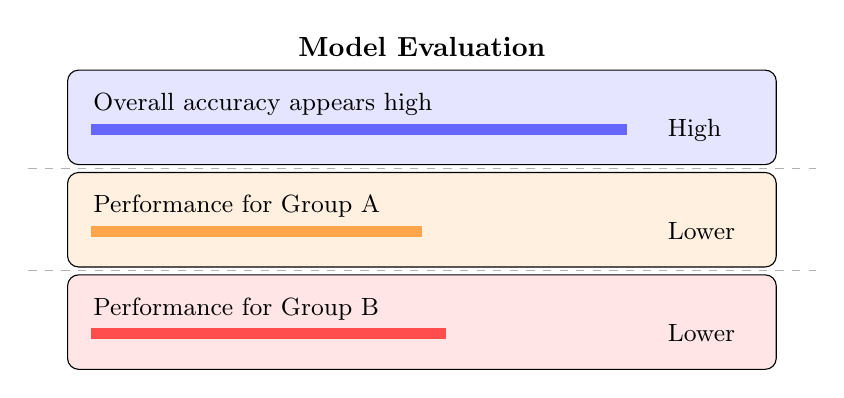
\begin{tikzpicture}[
    font=\small,
    box/.style={
        draw,
        rounded corners=4pt,
        minimum height=1.2cm,
        text width=9cm,
        inner sep=0pt
    }
]

% Title
\node[font=\bfseries] at (0,2.2) {Model Evaluation};

% Overall box
\node[box, fill=blue!10] (overall) at (0,1.3) {};
\node[anchor=north west] at ([xshift=6pt,yshift=-5pt]overall.north west) {Overall accuracy appears high};
\draw[fill=blue!60, draw=none] (-4.2,1.08) rectangle (2.6,1.22);
\node[anchor=west] at (3.0,1.14) {High};

% Group A box
\node[box, fill=orange!12] (groupa) at (0,0.0) {};
\node[anchor=north west] at ([xshift=6pt,yshift=-5pt]groupa.north west) {Performance for Group A};
\draw[fill=orange!70, draw=none] (-4.2,-0.22) rectangle (0.0,-0.08);
\node[anchor=west] at (3.0,-0.14) {Lower};

% Group B box
\node[box, fill=red!10] (groupb) at (0,-1.3) {};
\node[anchor=north west] at ([xshift=6pt,yshift=-5pt]groupb.north west) {Performance for Group B};
\draw[fill=red!70, draw=none] (-4.2,-1.52) rectangle (0.3,-1.38);
\node[anchor=west] at (3.0,-1.44) {Lower};

% Divider lines
\draw[dashed, gray!60] (-5,0.65) -- (5,0.65);
\draw[dashed, gray!60] (-5,-0.65) -- (5,-0.65);

\end{tikzpicture}
\caption{Overall accuracy can hide uneven performance across demographic groups.}
\label{fig:accuracy_bias}
\end{figure}


To address this, fairness metrics explicitly measure cross-group
performance differences. Metrics such as \emph{Equal Opportunity},
\emph{Equalized Odds}, \emph{Equalized Accuracy}, and \emph{FPR-based
disparity} provide a more nuanced understanding of model behaviour.
These metrics are formally defined in Chapter~\ref{ch:background} and
are used throughout this report for evaluation.

% ,,,,,,,,,,,,,,,,--
\section{Motivation for Fairness-Aware Learning}
\label{sec:motivation}
% ,,,,,,,,,,,,,,,,--

Recognising that bias is systemic and that aggregate metrics are
insufficient motivates the need for fairness-aware design. Traditional
approaches often rely on post-hoc corrections, such as calibration or
output reweighting. While useful, these methods are inherently reactive
and cannot address biases embedded within learned representations.

A more principled approach focuses on the representations themselves.
If the features learned by a model do not encode protected attributes,
then predictions derived from these features are less likely to exhibit
systematic bias. This idea forms the basis of \emph{fair representation
learning}, which aims to balance predictive utility with demographic
invariance.

However, achieving this balance is challenging. In real-world data,
target and protected attributes are often correlated. For example,
factors such as employment and housing stability may influence prediction
tasks while also being correlated with demographic characteristics.
Removing all demographic information risks discarding useful predictive
signals.

This trade-off between fairness and performance represents a central
challenge in modern machine learning. The goal is to reduce bias without
compromising accuracy, a problem that motivates the methods explored in
this report.

\subsection{Limitations of Prior Approaches}

Existing fairness methods are typically categorised based on where the
intervention occurs. \emph{Pre-processing} methods modify the data before
training, for instance by rebalancing datasets. \emph{In-processing}
methods introduce fairness constraints directly into the learning
objective. \emph{Post-processing} methods adjust predictions after the
model has been trained.

Each category has inherent limitations. Pre-processing may remove
informative features, reducing model performance. Post-processing cannot
eliminate bias embedded in internal representations. In-processing
methods, if not carefully designed, may fail to account for complex
dependencies between attributes.

A further limitation arises in disentangled representation learning.
Earlier approaches, such as FFVAE, partitioned the latent space into
``sensitive'' and ``non-sensitive'' components. However, due to
correlations between attributes, demographic information can still be
indirectly encoded in the non-sensitive subspace.

The FD-VAE framework addresses this limitation by introducing an
additional \emph{mutual} latent space that captures shared information
between target and protected attributes.

